\section{Costumer overview}
The problem in attaining broad coverage of use cases, and therefore completeness in requirements i primarily that, from the customer perspective, that they feel very overly-verbose and usually too formal in nature. For software engineers, the opposite is usually the case. They feel that the use case descriptions are not structured nor elaborate enough for use in, for instance, code stub generation.

More structure, however, could be helped along the way with proper tooling. Hiding some of the complexity of the constrains of a data model behind a simple user interface supplying dragable components and providing immediate visual feedback in the form of textual use case representation (or a diagram) could "cheat" the customer into adding the needed structure to the use case model.

\begin{figure}[h]
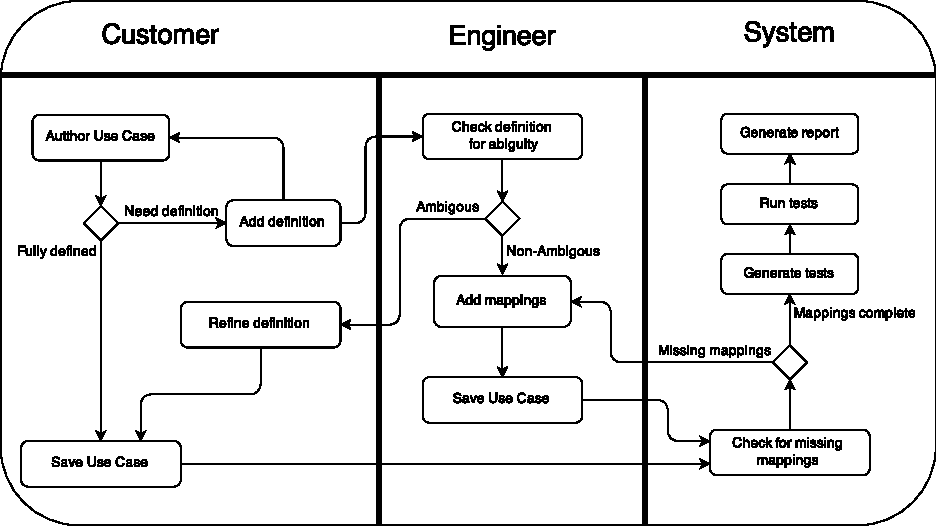
\includegraphics[scale=0.75]{img/use_case_creation_activity_diagram}
\centering
\caption{Use case creation with different actors}
\label{fig:use_case_creation_activity_diagram}
\end{figure}

What is in the customers interest is having acceptance tests match the use cases as closely as possible. Preferably, the should be able to be automated as well. Figure \ref{fig:use_case_creation_activity_diagram} shows an activity diagram involving three actors, the customer, the engineer and the system\footnote{Use case system}. In this diagram, the customer authors use cases while adding missing definitions not already in the tool. A definition is textual description of a concept which may be -- for instance -- an actor, role or action. This description is then given a unique name, that may correspond to a concept already found in the domain model. The domain model, if defined beforehand, could also be thought to be a part of the built-in declarations.

\begin{figure}[h]
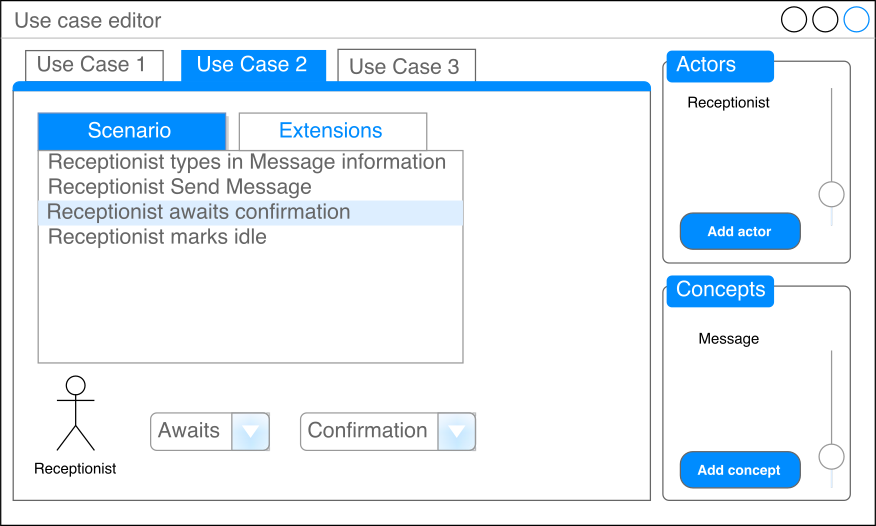
\includegraphics[scale=0.9]{img/test_case_ui}
\centering
\caption{Use case editor UI mockup}
\label{fig:use_case_editor_mockup}
\end{figure}

Whenever there is a new use case, a change to an existing use case, or simply a definition, the system should try to generate tests from the new information. If this step fails it is likely due to insufficient concept mappings. From here, a software engineer must manually map individual definitions to system macro-functionality or, possibly the use case could be linked to an existing manually written test, if the generation step is not possible for some reason. A mockup of a user interface from the customer point of view is shown in figure \ref{fig:use_case_editor_mockup}. A list of available actors (only containing one element, however) is shown on the right hand side. The main part of the window contains the use case currently being worked on. The bottom part of the window is the edit part, where dropdown lists of actions and targets resides.

\section{Brainstorm}
\section{Costumer overview}
The problem in attaining broad coverage of use cases, and therefore completeness in requirements i primarily that, from the customer perspective, that they feel very overly-verbose and usually too formal in nature. For software engineers, the opposite is usually the case. They feel that the use case descriptions are not structured nor elaborate enough for use in, for instance, code stub generation.

More structure, however, could be helped along the way with proper tooling. Hiding some of the complexity of the constrains of a data model behind a simple user interface supplying dragable components and providing immediate visual feedback in the form of textual use case representation (or a diagram) could "cheat" the customer into adding the needed structure to the use case model.

\begin{figure}[h]
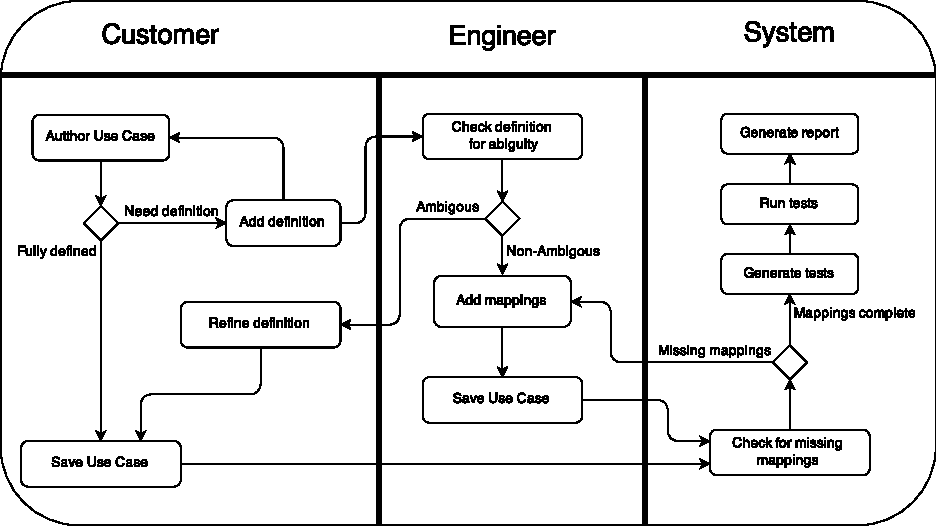
\includegraphics[scale=0.75]{img/use_case_creation_activity_diagram}
\centering
\caption{Use case creation with different actors}
\label{fig:use_case_creation_activity_diagram}
\end{figure}

What is in the customers interest is having acceptance tests match the use cases as closely as possible. Preferably, the should be able to be automated as well. Figure \ref{fig:use_case_creation_activity_diagram} shows an activity diagram involving three actors, the customer, the engineer and the system\footnote{Use case system}. In this diagram, the customer authors use cases while adding missing definitions not already in the tool. A definition is textual description of a concept which may be -- for instance -- an actor, role or action. This description is then given a unique name, that may correspond to a concept already found in the domain model. The domain model, if defined beforehand, could also be thought to be a part of the built-in declarations.

\begin{figure}[h]
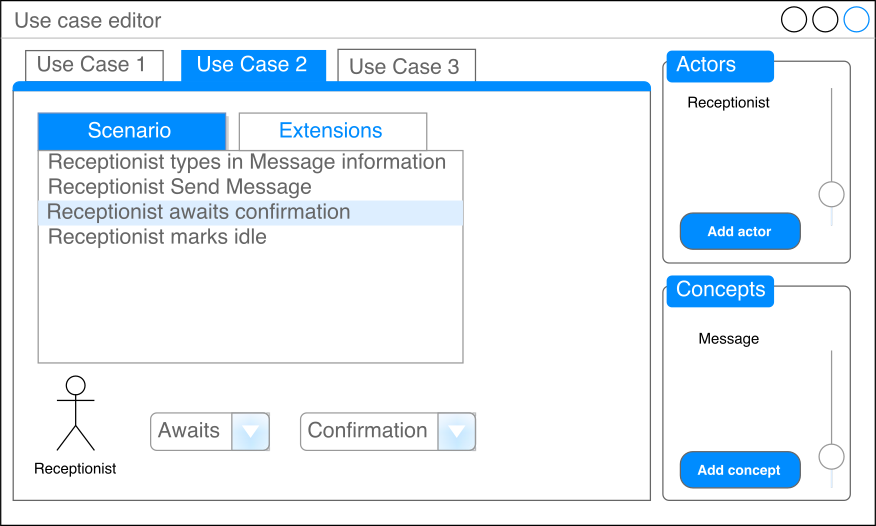
\includegraphics[scale=0.9]{img/test_case_ui}
\centering
\caption{Use case editor UI mockup}
\label{fig:use_case_editor_mockup}
\end{figure}

Whenever there is a new use case, a change to an existing use case, or simply a definition, the system should try to generate tests from the new information. If this step fails it is likely due to insufficient concept mappings. From here, a software engineer must manually map individual definitions to system macro-functionality or, possibly the use case could be linked to an existing manually written test, if the generation step is not possible for some reason. A mockup of a user interface from the customer point of view is shown in figure \ref{fig:use_case_editor_mockup}. A list of available actors (only containing one element, however) is shown on the right hand side. The main part of the window contains the use case currently being worked on. The bottom part of the window is the edit part, where dropdown lists of actions and targets resides.


\section{Proposed solution}
"Side-cart" tool that (maybe) uses natural language processing. The developement is supported by a two-sided approach. Both top-down and bottom-up. Meaning that design an implementation will go hand-in-hand and hopefully lead to a good middle-road.
%TODO something about existing approaches.
%TODO Step-wise go through the enhancement process.
%  - Basically, autogenerate the use case action code line
%  - Infer some Class dependencies, which then becomes Framework dependencies.
%Definition dictionary
% Remember that an actor has a set of goals, which he/she wants to realize through the system. Actor can be  primary (typically people) or supporting (provides service or information) - passive.
% A good goal has a verb/noun combination.
%REMEMBER TO TAKE INTO ACCOUNT <INCLUDE> use cases -- Basically extensions
This section takes starts from a use case description, and tries to go through the steps needed to convert it into an acceptance tests. The use case used in this text is simplified and outlined in verbatim text seen in listing \ref{lst:uc-simple-example}.\todo[inline]{Check context, and make sure it leads in to this.}.
\begin{lstlisting}[frame=single,style=usecase, caption=Use case example, label=lst:uc-simple-example]
Scenario:
  Receptionist types in message
  Receptionist sends message
  Receptionist marks state as ready 
Preconditions:
  The receptionist is created
  The receptionist is logged in
Postconditions:
  The message is stored
  The receptionist is ready to handle the next call
\end{lstlisting} 
Translating this example, we first identify the domain concept contained within the statements in the text. In this case, we here observe that it includes the concept ``message'' a ``receptionist'' actor. additionally; some interaction between the message and the actor, which we define as actions.\\
In listing \ref{lst:uc-simple-example-highlighted} we have highlighted the different parts of the use case, using an orange color for actors, green for actions, blue for domain concepts, and a dark red for attributes. Using this highlight, it illustrates the abstract interpretation and the interaction between the different part very well. It also reveals very clearly which archetype (actor, concept \dots) each of the different parts should have. 
\todo[inline]{More elaborate text here}.
\begin{lstlisting}[frame=single,style=usecase, caption=Use case example with its different parts highlighted, label=lst:uc-simple-example-highlighted]
Scenario:
  @\color{orange} Receptionist@ @\color{dkgreen}{types in}@ @\color{blue}{message}@
  @\color{orange} Receptionist@ @\color{dkgreen}{sends}@ @\color{blue}message@
  @\color{orange} Receptionist@ @\color{dkgreen}{marks state}@ as @\color{blue}{ready}@
Preconditions:
  The @\color{orange}receptionist@ is @\color{dkred}logged in@
Postconditions:
  The @\color{blue}message@ @\color{dkred}is stored@
  The @\color{orange}receptionist@ @\color{dkred}is ready@ to handle the next call
\end{lstlisting} 
Based upon the information in listing \ref{lst:uc-simple-example-highlighted}, we could create an abstract interpretation that generates a test that looks like listing \ref{lst:uc2_example_test_code}.
Each of the concepts in this example is mapped to a class, that could likely be stubbed out automatically by the test tool.\\\\
Given the amount of information in (and markup of) the use cases, we can easily generate code such as the one shown in listing \ref{lst:uc2_example_test_code}. But these functions are still very high-level, and doesn't assert anything about the system being tested. To do this, we need to fill in the methods used on our receptionist and message object.
\begin{lstlisting}[caption=Suggestion of generated test case,label={lst:uc2_example_test_code}]
boolean test (receptionist, message) {
  // Scenario
  receptionist.types_in (message);
  receptionist.sends (message);
  receptionist.marks_state (idle);
  
  // Postcondition
  return
    message.is_stored() AND
    receptionist.is_ready();
}
\end{lstlisting}
Going through the test case, from the top, we can see that the \texttt{receptionist.types\_in~(message)} method operates on the receptionist actor call, and requires knowledge of the ``message'' domain concept. Furthermore, we known from the domain analysis that \emph{is not part} of the use case, that the action of typing in a message is actually a creation of message. So, before being able to test it, we need some way of simulating the message creation and -- more concretely -- fill in the actual message content. Conceptually, this is some sort of content generator. A concrete implementation could be a simply ``dummy object'' or an object that is initialized with random content. Once the message object is mapped to a content generation function, we will be able to fully generate the test. The content generation function would probably still need to be hand coded, as this is example data.\\\\
The next statement; \texttt{receptionist.sends (message)} can be classified as a store function. It takes the argument ``message'' and makes it available for other actors to access later on, by storing it persistently. This is typically done using a database or file store. By mapping a message to a message store, we can remap an ``enqueue'' method of the message object, which needs to have a notion of where it is, or should be stored. This is realized by having a ``messageStore'' interface which is a service interface object that, can actually be originating directly from the code base of the system under test.\\\\
The final statement in the scenario is \texttt{receptionist.returns\_to (ready\_state)}. This is actually a mutation function that alters the state of the receptionist actor. This state change could be global and should then  be updated multiple places, which then leads to additional ``state-store'' dependencies. Here, we also note that there is a concept of a ready\_state this is an explicit state change that could, possibly be linked to a state machine contained within the receptionist actor object.\\\\
The final thing done in the tests, is the postconditions. In this case, we treat the postcondition as a boolean attribute of the concept which it refers to. The general assumption is that pre- and postconditions are expressions that must always be true, and must refer to a concept previously referred to in the scenario. So for the \texttt{receptionist.is\_ready()} predicate we can map it to the internal state of the receptionist being equal to the ``ready'' state.\\\\
The mapping can be described in a textual language such as shown in listing \ref{lst:mapping_language_concept} where we initially state the domain concept name -- which is in this case Receptionist -- and the requirements, properties and mappings it has, plus which functionality it provides. The requirements are which other domain concepts are needed by this one. The properties are the boolean properties that are used in predicates and the ``provides'' section are functions that are either used as internal auxiliary functions, or exported functions that other concepts may use.
%Prior to running the tests, the two objects ``message'' and ``receptionist'' needs to be initialized.
%The question is then how much more needs to be added. Can we use some stereotyping to increase the semantics of the annotated use cases? Such as 'storage' for message, and 'actor' for receptionist.
%So last question; who does what, and how much can be automated?
%The first part of the job; typing in the use cases is a manual process that should be done in close cooperation with -- and preferably by -- the stakeholder involved in the use case. So a use case involving an accountant actor should be typed by a accountant representative expected to be using the system, once finished.

\begin{lstlisting}[caption=example language for mapping concepts,label={lst:mapping_language_concept}]:
Receptionist:
  requires:
    MessageContentGenerator messageContentGenerator
    ReceptionistState currentState = ReceptionistState.Unknown
  
  provides:
    changeState (ReceptionistState rs) -> currentState = rs
  
  maps:
    sends_message (Message msg) -> msg.enqueue()
    types_in (Message msg) -> msg.content = messageContentGenerator.next().content
    returns_to (ReceptionistState newState) -> this.changeState (newState)

  properties:
    is_ready -> receptionistState == ready
\end{lstlisting}
The mappings are, in this conceptual model, alias functions to ``real methods'' already provided in the code base of the software under tests, or to functions of other domain concepts. This is probably not feasible in praxis, and will probably be a programing code template instead.

\begin{lstlisting}[caption=Pseudo code representing Receptionist domain actor,label={lst:code_for_receptionist_domain_actor}]
class Receptionist {
   MessageContentGenerator messageContentGenerator= ...;
   ReceptionistState receptionistState = ...;
  
  void types_in (message) {
  	message.updateContent(messageContentGenerator.content);
  }
  
  void sends (Message message) {
    message.enqueue();
  }
  
  // Alias function.
  void returns_to (State newState) {
  	changeState (newState);
  }
  
  void changeState (State newState){
  	receptionistState = newState;
  }
  
  boolean is_ready() {
    return receptionistState == ready;
  }
}
\end{lstlisting}

\begin{lstlisting}[caption=Pseudo code representing Message domain concept,label={lst:code_for_domain_concept}]
class Message {
  RESTMessageClient messageStore = ...;
  
  void enqueue() {
    messageStore.enqueue(message);
  }

  boolean message.is_stored() {
    messageStore.contains(this);
  }
}
\end{lstlisting}

\begin{figure}
 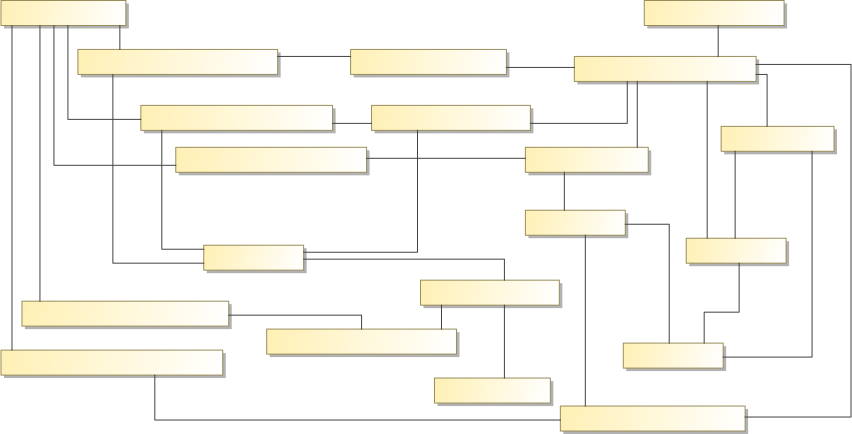
\includegraphics[scale=0.45]{img/uc2_test_config}
 \caption{Object diagram showing the use case as mapped test}
\end{figure}
The function mappings are done in the current solution, by manually writing up the logic needed in a support library, that in many situations reuse the framework directly. For instance, for every service, we have made a client class that, similar to RMI or WSDL handles all the low-level serialization and deserialization work. 

This enables us, in our tests to merely require that an interface (a client of it, that is) is provided to use, rather than having to explicitly elaborate the code in the test case.

%TODO Brief discussion on randomizers.

\begin{figure}
 \centering
 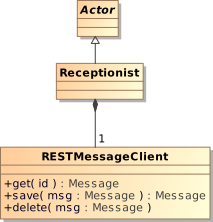
\includegraphics[scale=0.60]{img/support-tools-recepionist-example}
 \caption{support-tools-recepionist-example}
 \label{fig:support-tools-recepionist-example}
\end{figure}

%\begin{figure}
% \centering
%\missingfigure[figwidth=6cm]{This is some text that is with the todo and in the figure}
% \caption{support-tools-recepionist-example}
% \label{fig:support-tools-recepionist-example}
%\end{figure}

\begin{figure}
  \centering
 
  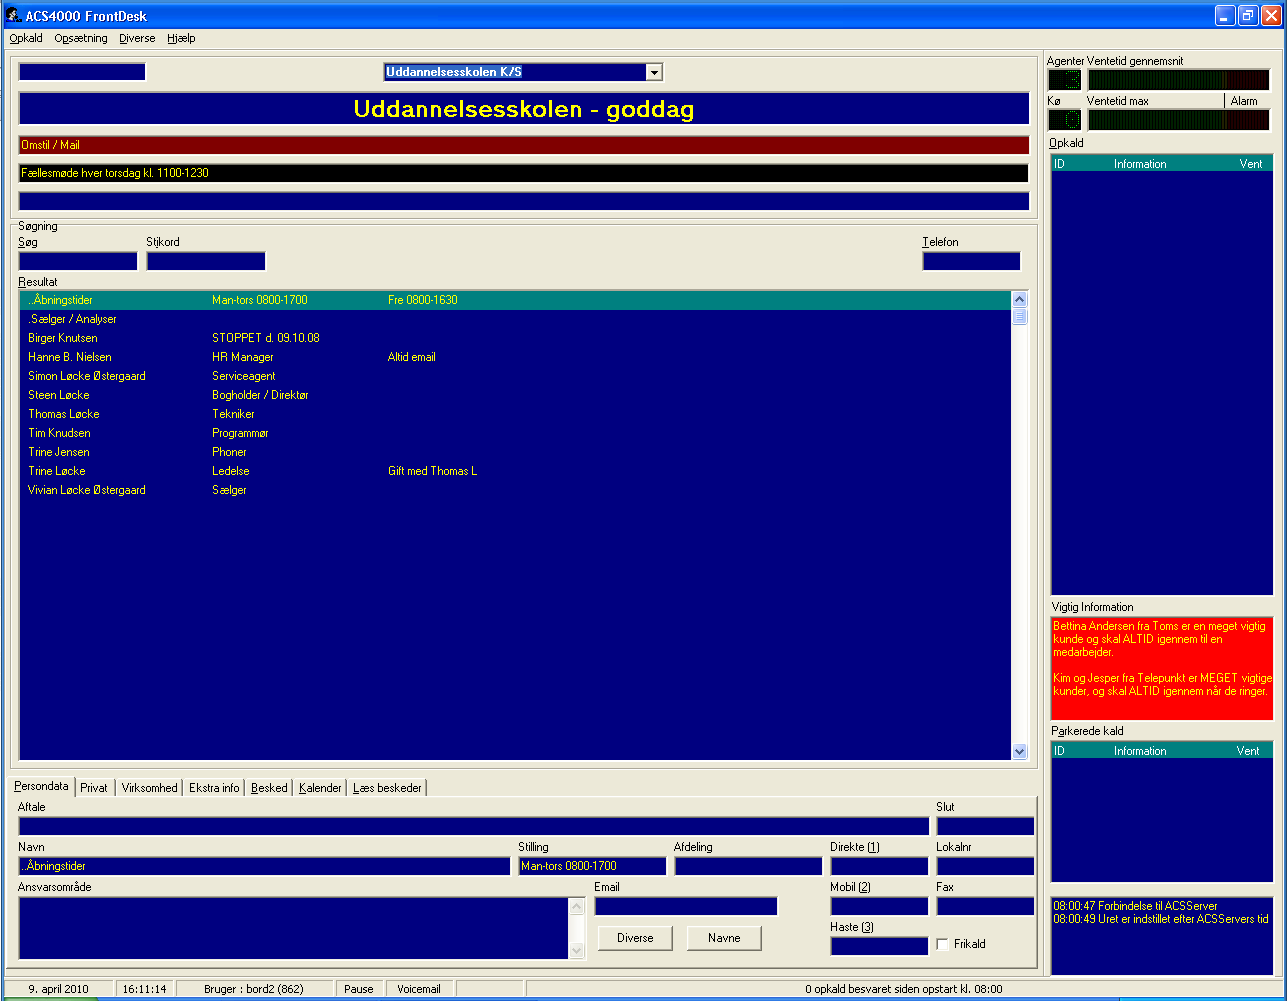
\includegraphics[scale=0.2]{img/frontdesk-client-ui.png}
  \caption{Receptionist client user interface of existing system}
  \label{fig:frontdesk-client-ui}
\end{figure}

\begin{figure}
  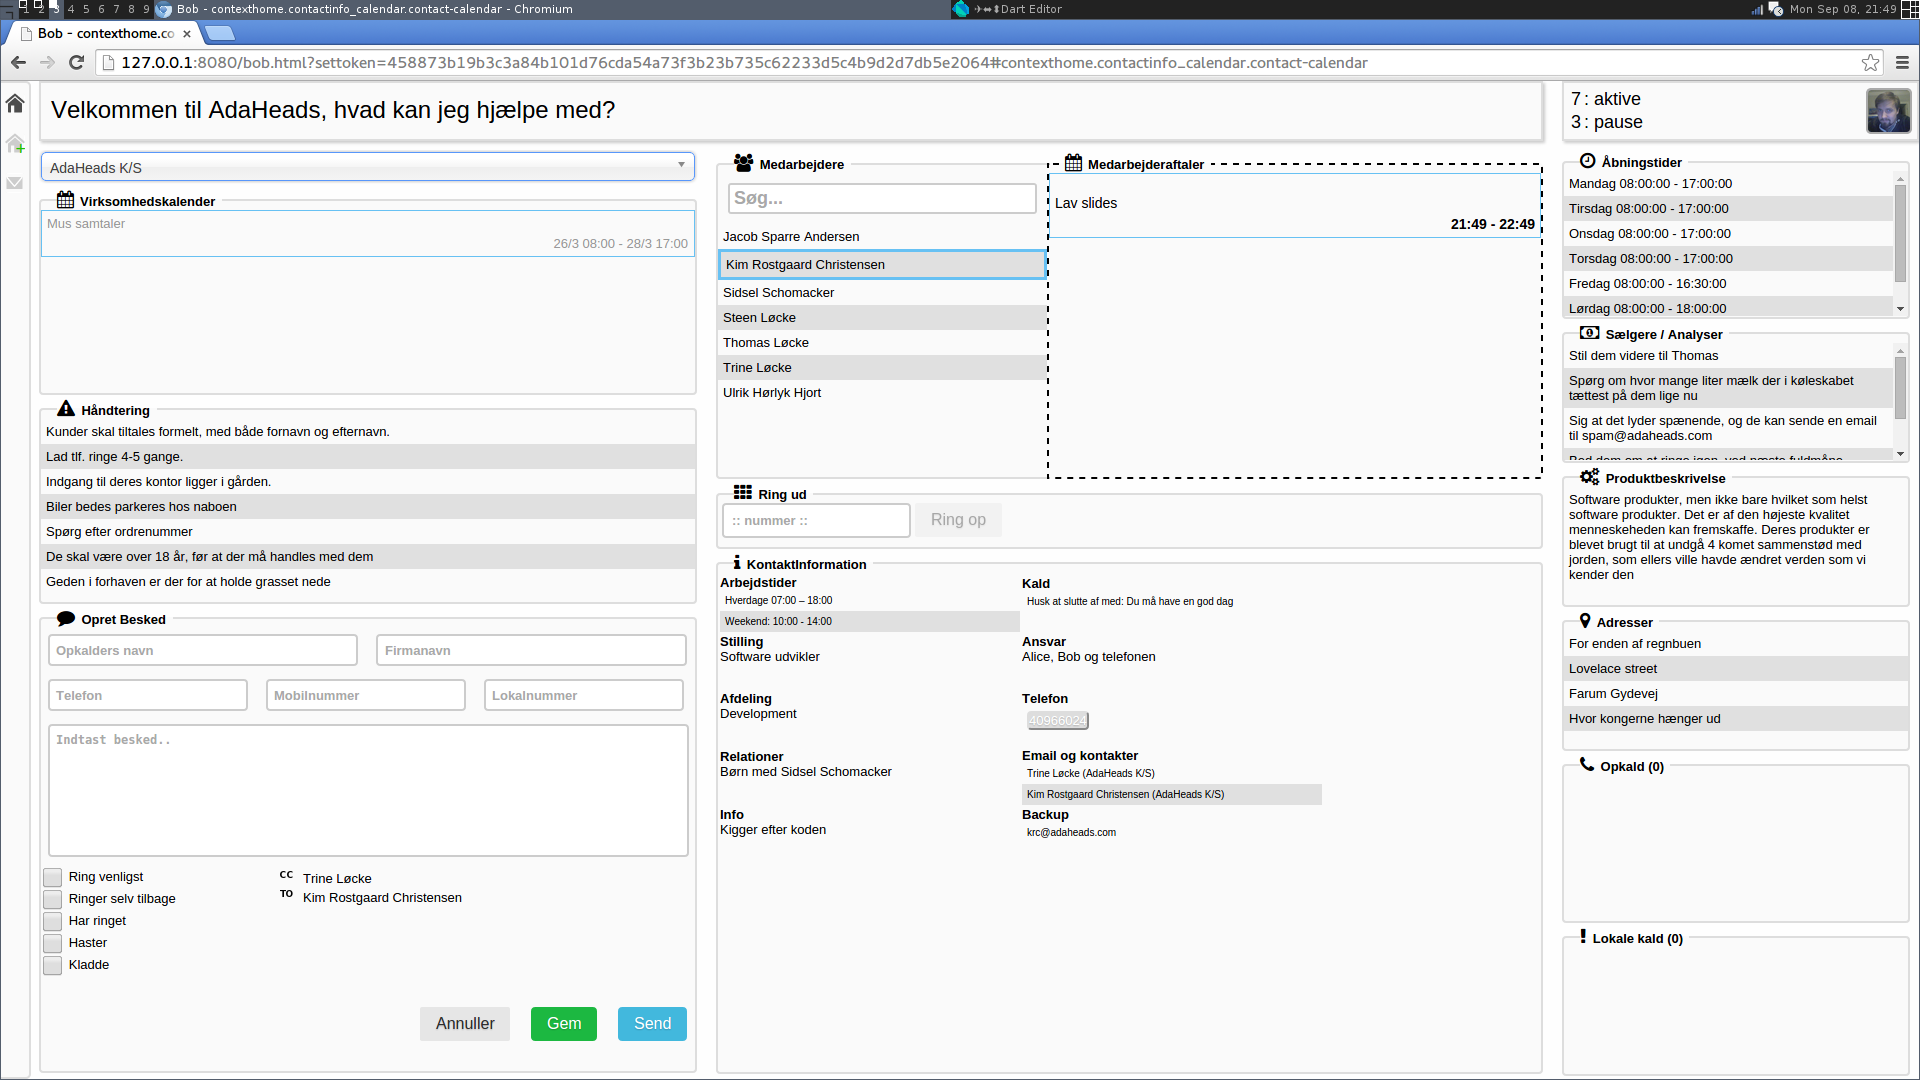
\includegraphics[scale=0.2]{img/openreception-client-ui.png}
  \caption{Receptionist client user interface of OpenReception system}
  \label{fig:openreception-client-ui}
\end{figure}

\begin{figure}[h]
%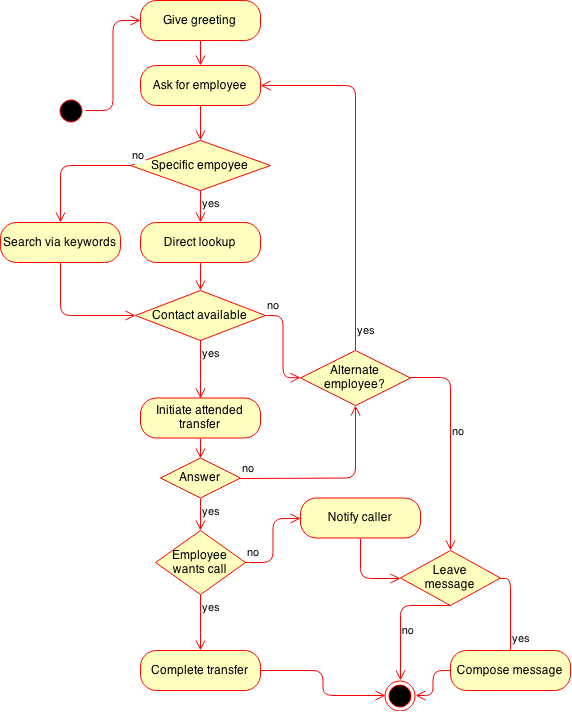
\includegraphics[scale=0.4]{img/activity_diagram_receptionist}
\centering
\caption{Activity diagram for the receptionist actor}
\label{fig:activity_diagram_receptionist}
\end{figure}


%\section{Related work}
%\subsection{Writing requirements as tests}
%\subsection{Writing requirements in formal language}

\section{Brainstorming}
The problem in attaining broad coverage of use cases, and therefore completeness in requirements i primarily that, from the customer perspective, that they feel very overly-verbose and usually too formal in nature. For software engineers, the opposite is usually the case. They feel that the use case descriptions are not structured nor elaborate enough for use in, for instance, code stub generation.

More structure, however, could be helped along the way with proper tooling. Hiding some of the complexity of the constrains of a data model behind a simple user interface supplying dragable components and providing immediate visual feedback in the form of textual use case representation (or a diagram) could "cheat" the customer into adding the needed structure to the use case model.

\begin{figure}[h]
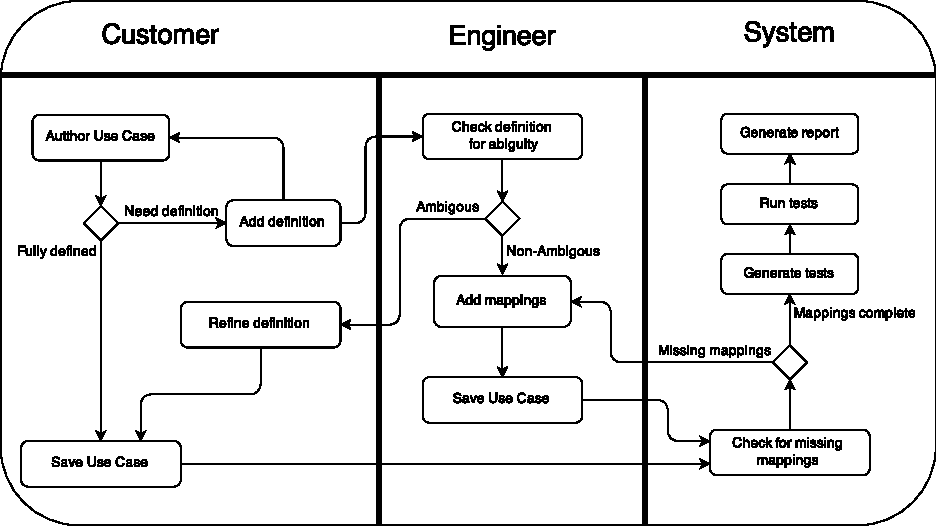
\includegraphics[scale=0.9]{img/use_case_creation_activity_diagram}
\centering
\caption{Use case creation with different actors}
\label{fig:use_case_creation_activity_diagram}
\end{figure}

What is in the customers interest is having acceptance tests match the use cases as closely as possible. Preferably, the should be able to be automated as well. Figure \ref{fig:use_case_creation_activity_diagram} shows an activity diagram involving three actors, the customer, the engineer and the system\footnote{Use case system}. In this diagram, the customer authors use cases while adding missing definitions not already in the tool. A definition is textual description of a concept which may be -- for instance -- an actor, role or action. This description is then given a unique name, that may correspond to a concept already found in the domain model. The domain model, if defined beforehand, could also be thought to be a part of the built-in declarations.

\begin{figure}[h]
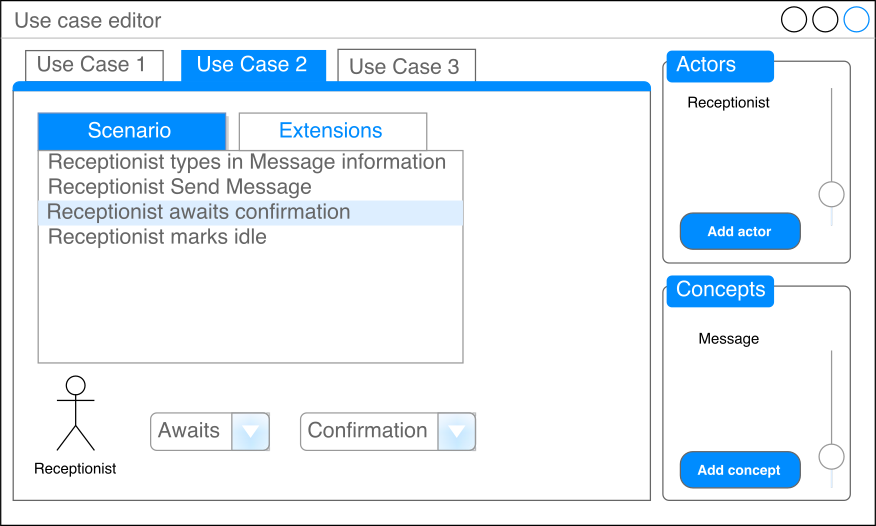
\includegraphics[scale=0.9]{img/test_case_ui}
\centering
\caption{Use case editor UI mockup}
\label{fig:use_case_editor_mockup}
\end{figure}

Whenever there is a new use case, a change to an existing use case, or simply a definition, the system should try to generate tests from the new information. If this step fails it is likely due to insufficient concept mappings. From here, a software engineer must manually map individual definitions to system macro-functionality or, possibly the use case could be linked to an existing manually written test, if the generation step is not possible for some reason. A mockup of a user interface is shown in figure \ref{fig:use_case_editor_mockup}.

% Something about generating partially-automated tests, where the system sets up everything for the customer and then notifies them about the next steps they have to take to move the test forward.

\section{Extracting semantic}
Example; in the use case it is stated that a call is hung up and a callee awaits this event. The lifeline of the call is however not tracked and to be able to properly assert the true state of this, the code macro needs to into account this lifeline and reflect on which assertions hold for every stakeholder that has knowledge of the call. % TODO: Elaborate the example and explain that a phone call is a good example because it has an A and B-leg and potentially a system that tracks its state.

\subsection{Letting the customer inject semantics}

There are two basic approaches to letting the customer inject semantics into the requirements. The first is to do a full up-front declaration of every term used within the problem domain and supply this as a toolbox for the customer %todo example.
The other approach is to do it on the go by outlining concepts as stubs whenever they appear. This approach is similar to what is used in wiki software. %todo eaxmple

\section{Class-responsiblity-collaboration cards}
%Nouns should turn into the classes of the card, verbs typically turn into the responsibilities of the card, and collaborators are the other cards with which the card will be interacting with.
%FROM: http://en.wikipedia.org/wiki/Class-responsibility-collaboration_card

\section{Verification problem}
A big issue in software

\section{End-user experience}
%The challenge in documenting requirements is, and has always been, to formulate them on a non-ambiguous form. The quantification of ambiguity tends to be difficult as well, due to the fact that requirements are usually formulated in natural languages following some rules, such as pre-defined glossary and constraints. Constraints vocabulary typically consists of should, could, may, must.

%As requirements are basically constraints to your system, a subset of them may be expressed as expressions following a formality that is machine-interpretable. Vienna Development Method (VDM) and Z notation are two approaches that tries to formally describe systems on a very high level, so that model-checking can be performed on it prior to programming.

An example UI is Starting from scratch, the user would be expected to initially define at least one actor and add a sequence of actions that the actor perform.

%Other method
Wiki-collaboration to "lazily" define the problem domain and verification conditions along the way.

\section{Test setup}
%scaffolding and harness

\section{Formulating requirements}

\section{Framework discussion}
\subsection{Metrics}
% How many lines of code is the support tools? The middleware framework?
% How is it compared to the activity count in the activity diagram?
\subsection{Recommended test framework guidelines}
%Use allocation pools
%Use interfaces a objects.

\section{Requirements as communication platform}

Avoid technical jargon (\cite{christel1992issues})

\section{Related work}
\subsection{FIT Framework}

We've taken an offset in use cases, but there could be other ways of structuring the requirements of a system, such as the SCRUM user story format;
%Use the SCRUM approach. Don't describe a feature as
%"It should be doing this and that in the following way"
%While the sentence above describes all you need to know to implement the feature, it does not justify the feature. My SCRUM book says features should be written down as a story. A story looks like this:
%"As a <user-role>
%I need a <functionality>
%So that I get <business value>"
%A feature that cannot be justified using such a story is an unjustified feature and thus there is no use to actually implement it.
%E.g.
%"As a visitor of a web portal I need a way to authenticate, so I can access my customer data, but nobody else can"
%Now you don't only know that you need an authentication for your web portal, you also know who needs it (the visitors, basically everyone planing on using it more intensively) and you also know why it is needed, as it gives the user some value.
%Other examples:
%"As a passenger I need a list of all my booked journeys, so that I know when I'm going to travel where and won't lose the overview"
%"As a book keeper, I'd like to have the sales tax being automatically printed to each bill based on customer data, so that I don't have to enter it manually each time I'm printing a bill"
%If every feature needs to be written like that, you'll automatically see if a feature is for the customer, because it is really necessary, or just something your boss/company wants to have and also why they want to have it (what is the big picture behind it? Why are they doing it?).


\section{Use case writing level}
Should not be used to describe UI actions% http://alistair.cockburn.us/Use+cases%2c+ten+years+later (Use case limits).

Use cases expresses expected system behavior. Keep use cases free of UI-action.

There are several levels on which use cases can be written as per\cite{cockburn??}. In our case, it would make the most sense to use the "system" level, as business level is something that is nearly useless because it is largely out of scope. The business logic is also, more elaborately (and implicitly) formulated within a system-level use case. In the other end, a component use case is also very impractical, as our target audience would be people that does not know anything about the specifics of the system being built.

%Note;
An important aspect to keep in mind is that context is important. Writing hundreds of pages of detailed requirements are bound to be decoupled and lose context, and coherence with each other. Deciding on a level that keeps context is important.

\section{Expressing requirements}
%Requirement gathering and documentation often feels a lot like stating the obvious, and being overly-verbose.

\section{Use case translation}
%TODO Add a section on multiple actors and race conditions. How do you create a use case that contains multiple simultanious instances of actors that perform the same action synchronously? Basically asserting parallel properties.

This section tries to extracts an abstract interpretation of a use case through a brief study of two use cases. The goal is to come up with a meta-model of use cases that captures the essentials of the informally written use case, and allow us to map the concepts from it to an abstract syntax so that test code may be generated from it.
\section{Use case semantics}
In order to help the computer make more sense of our use cases, we need to define to it what a use case is. But since a use case is neither strictly defined nor standardized anywhere, we need to pick a suitable representation.
To help us extract some machine-understandable structure -- or merely semantics -- of use cases, we've hand-picked two use cases from our case study system.\\\\
The first use case is a basic phone call forwarding session that goes though a receptionist. The use case is described from the receptionist's point of view, as this is the scope of the main case study system. The use case has a detailed description in schema form in figure \ref{fig:uc1}. \\\\
The second use case is, in a sense, embedded in the first one as it part of the extensions of that use case. This will be covered later on. The use case covers a ``send message'' session typically done by having the receptionist actor transcribe a spoken message along with caller information (name, company, ...) onto a set of text input fields that then can be assembled to a message. This message is then handed over to the system that may enqueued it for later delivery -- or send it immediately, depending on implementation.

\subsection{Identifying concepts}
The first concept we know, for certain, should got into our meta model is the use case. It serves as our top-level concept that every other concept, in some way, relates to. From here on, we go back to our two case study use cases use cases where we can easily -- by manual inspection -- identify various concepts that most likely also belongs in a domain model. In use case 1 (figure \ref{fig:uc1}), we see three different actors: A receptionist, a contact and a caller. We also have a primary actor that provides us with the ``glasses'' we see the use case through. This, in conclusion, means that we need an actor as part of our domain model, and an association between a use case and an actor.\\\\
Skipping the pre- and postconditions for now, we take a look at the ``Main success scenario'' and see that, broadly speaking, each use case action involves one actor performing an action, possibly affecting a target object -- which could be another actor. For the purpose of generating tests, it is not important that actors may target other actors though their actions, and this association is therefore left out of the meta model.\\\\
Given the loose structure of the use case concept, we believe it is sufficient to treat preconditions as simply other use cases. A more elaborate motivation for this can be found in section \ref{sec:test_case_state}.\\\\
Postconditions are defined to be predicates. This is because they share the common trait that they must be true, for the given expression to be true. In our case, the postcondition ``Receptionist is ready for next call'' states the actor receptionist that is participating in this use case, must be in a specific state when the last statement of the use case is done. A postcondition should refer to an actor, target or action previously defined in the use case to avoid redundant mapping. The predicate itself can be some sort of quantifiable strict logic such as ``Message has recipients'', or could as an extension be defined as the more loose ``Message should have recipients'', which should map to a warning in the generated tests, rather than an error.

Pre and post-conditions are operations that work on expressions rather than statements

Alternate scenarios are not yet covered.

\subsection{Meta model}
This section contains a brief discussion of a meta model that could be used for translating use cases into test cases. The discussion is supported by the graphical model depicted in figure \ref{fig:meta_model}\\\\
Within the definition mapping, the mapping class denotes the relation between either a predicate and a predicate expression, or a statement (indirectly by the actor, action, target composition). The mapping is uniquely defined by mapping by its composition of an actor, an action and a target, as it should be safe to assume that ``The contact accepts the call'' means the same no matter which use case it appears in. Each mapping will imply a requirement on a resource, which can be any actor or target. The are basically constraints stating the minimum functionality the test framework\footnote{Domain-specific scaffolding code that needs to be written by hand} should have to make the generated test code runnable. These resources could, in test code frameworks, be provided by factory classes or object pools.\\\\
Tests are the output of a sequence of mappings, that has a state which is then defined by the mappings that originally defined the test. The test will also have references to the predicate expressions that are outputted by mappings as well.

\begin{figure}[h]
  \centering
 
  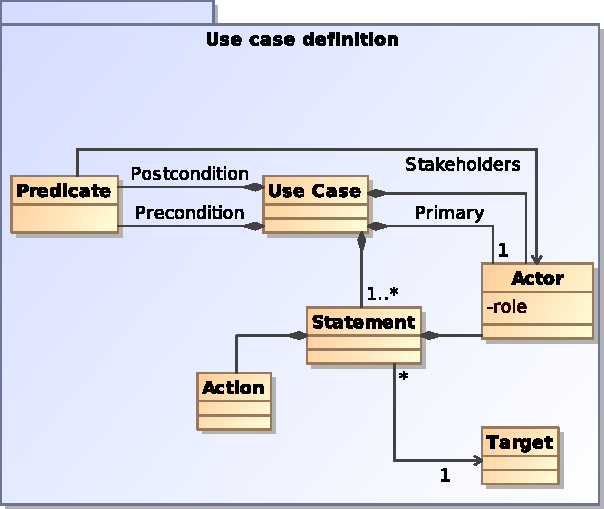
\includegraphics[scale=0.72]{img/use_case_meta_model}
  \caption{Intermediate meta model for use case representation along with tests}
  \label{fig:use_case_meta_model}
\end{figure}

\begin{figure}[h]
  \centering
 
  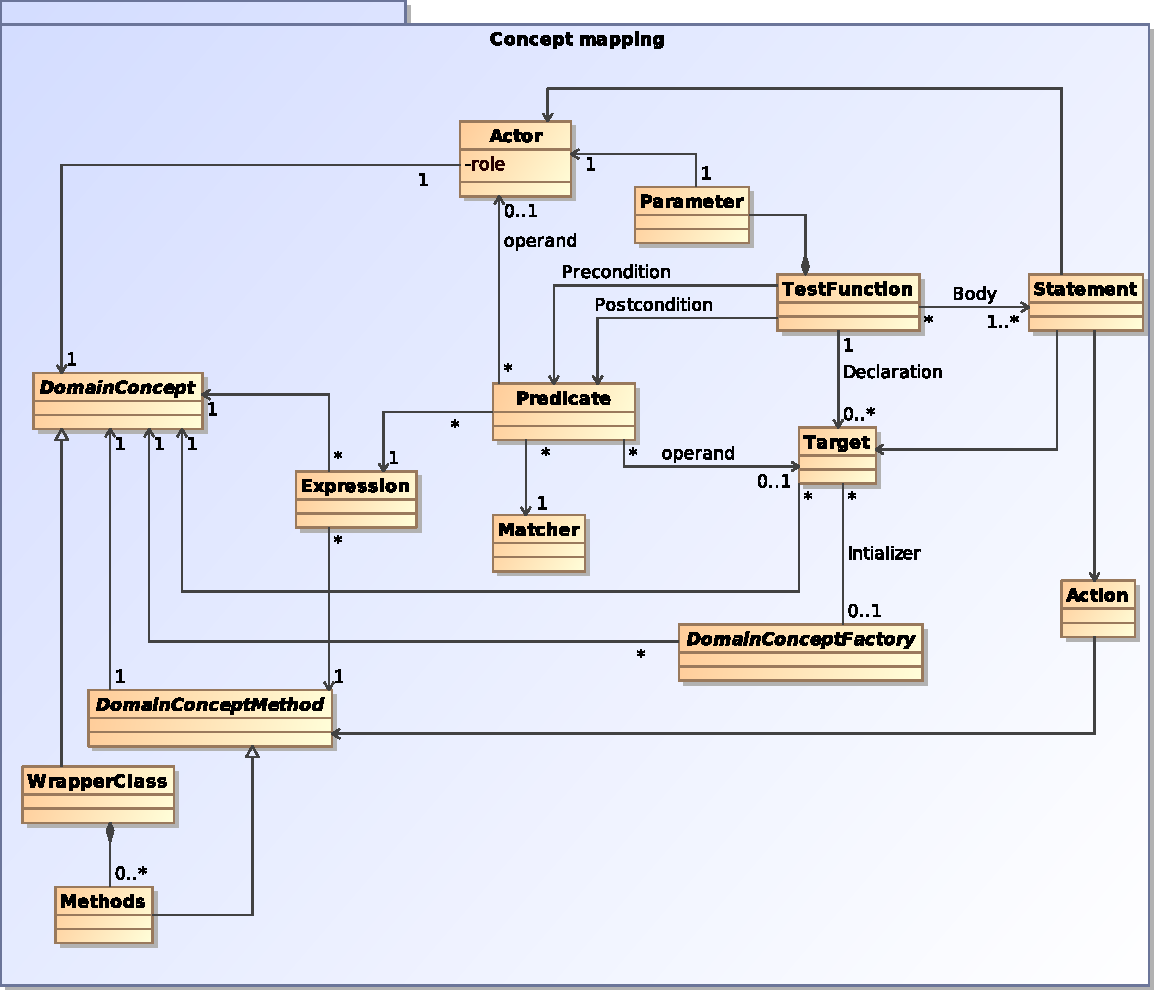
\includegraphics[scale=0.72]{img/use_case_mapping}
  \caption{Use case mapping}
  \label{fig:use_case_mapping}
\end{figure}

\section{Mapping manually}
Within a use case there are some bits of implicit knowledge that we need to extract. To begin with, we observe that for the use cases in figure \ref{fig:uc1} and \ref{fig:uc2}, there are domain actors involved.

Each involved domain actor will then be mapped to a wrapper class that represents the domain object, and could possibly extend a class from the implemented code base.

In order to get the actor object to perform actions, we need to map the actions in the use case to some functions associated with the actor class. These functions could be a direct link to a method that is part of the main codebase which is tested against, a new method written specifically for this purpose - or a macro function that combines functionality from different domain concepts in a single functions.

Whenever there is a mention of an object (a target of an action) which could be, for instance, a message object we assume that its the same object that is tracked during the entire use case. So, from use case 2, we have ``Receptionist sends the message via the system'' in the main success scenario and ``Message is stored and ready for dispatching'' in the postconditions.

Regarding the test as a function

%\section{Object tracking} NOTE: Maybe something about object lifecycles (and statemachines for them) here.

\section{Test case state}
A test consists of three basic steps; setup, run and teardown. Setup and teardown is different from pre- and postcondition in that they are unrelated to the test itself, they merely make sure that objects are initialized with right values and, in general, are in the state that the test expects.

There needs to be an executable domain model programmed, not necessarily complete, but the concepts covered in the use cases should at least be there. So for \ref{fig:uc2}. We need at least a class representing the actor ``Receptionist'', and a class representing a message. The actions performed by the actor could then either be class methods, or simply functions taking the primary actor (or more exact; classes of the actor), as an argument.


%NOTE: The test mapper will then select the "essentials" of the sentence, which could be just the verb, noun and object.
\label{sec:test_case_state}


\section{Test case example}
\begin{lstlisting}
void use_case_1 (Receptionist receptionist) {

   MessageObjectFactory messageObjectFactory = new MessageObjectFactory();
   Message message = messageObjectFactory.create();

   // Preconditions
   Matcher.has (selected_contact (receptionist));

   // Use case body 
   receptionist.types_in(message);
   receptionist.sends(message);
   receptionist.marks_state_idle();

   // Postconditions 
   Matcher.is_true (is_stored (message));
   Matcher.is_true (is_idle (receptionist));
}
\end{lstlisting}

\begin{figure}
  \centering
 
  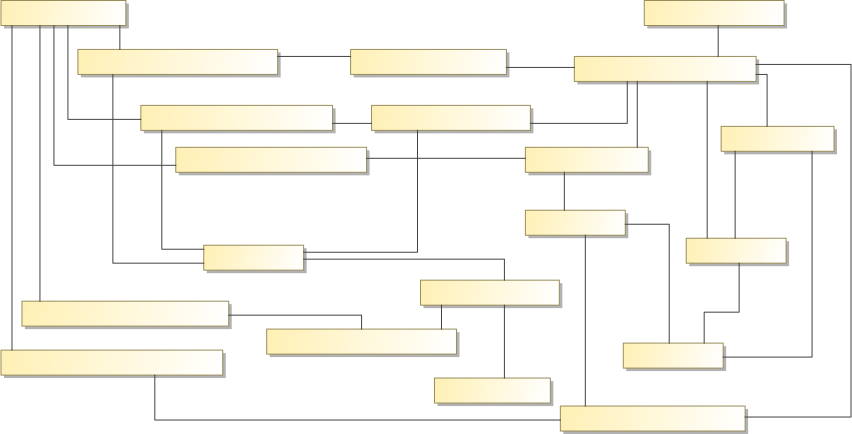
\includegraphics[scale=0.6]{img/uc2_test_config}
  \caption{object diagram depicting the configuration of use case 2}
  \label{fig:uc2_object_diagram}
\end{figure}


\begin{figure}[h]
  \centering
\begin{usecase}

\addtitle{Use Case 1}{Transfer to contact} 

%Scope: the system under design
\addfield{Scope:}{System-wide}

%Description: A brief description of the use case
\addfield{Description:}{The receptionist actor must be able to transfer an active call to a chosen -- dialed -- contact associated with the currently active reception}

%Level: "user-goal" or "subfunction"
\addfield{Level:}{User-goal}

%Primary Actor: Calls on the system to deliver its services.
\addfield{Primary Actor:}{Receptionist actor}

%Stakeholders and Interests: Who cares about this use case and what do they want?
\additemizedfield{Stakeholders and Interests:}{
	\item Receptionist: Wants to process the call with regards to the caller's wishes
	\item Caller: Wants to reach a specific contact
}

%Preconditions: What must be true on start and worth telling the reader?
\additemizedfield{Preconditions:}{
      \item Receptionist has picked up incoming call from caller
      \item Receptionist has parked incoming call
}
%when multiple
%\additemizedfield{Preconditions:}{} 

%Postconditions: What must be true on successful completion and worth telling the reader
\additemizedfield{Postconditions:}{
      \item Caller and contact's phones are connected
      \item Receptionist is no longer in call and ready for next call      
}
%when multiple
%\additemizedfield{Preconditions:}{}

%Main Success Scenario: A typical, unconditional happy path scenario of success.
\addscenario{Main Success Scenario:}{
      \item Receptionist dials a number of the selected contact
      \item The contact accepts the call (picks up)
      \item Receptionist has a dialogue with contact
      \item Receptionist transfers contact to caller
      \item Receptionist marks his/her state as idle.
}

%Extensions: Alternate scenarios of success or failure.
\addscenario{Extensions:}{
	\item[2.a] Contact cannot be reached
		\begin{enumerate}
		\item[1.] Receptionist tries alternate contact
		\item[2.] Receptionist returns to step 1
		\end{enumerate}
	\item[3.a] Contact declines transfer
		\begin{enumerate}
		\item[1.] Receptionist hangs up contact
		\item[2.] Receptionist picks up caller
		\item[3.] Receptionist offers caller to leave a message
		\item[4a.] Caller wishes to leave a message
		\begin{enumerate}
			\item[1.] Receptionist types in message and caller information
			\item[2.] Receptionist saves message
		\end{enumerate}
		\item[4b.] Caller does not wish to leave a message
		\item[5] Receptionist ends call with caller
		\item[6] Receptionist returns to step 6
		\end{enumerate}
}

%Special Requirements: Related non-functional requirements.
%\additemizedfield{Special Requirements:}{
%	\item first applicable non-functional requirement
%	\item second applicable non-functional requirement
%}

%Technology and Data Variations List: Varying I/O methods and data formats.
%\addscenario{Technology and Data Variations List:}{
%	\item[1a.] Alternative first action with other technology
%}

%Frequency of Occurrence: Influences investigation, testing and timing of implementation.
%\addfield{Frequency of Occurrence:}{}

%Miscellaneous: Such as open issues/questions
%\addfield{Open Issues:}{}

\end{usecase}
   \caption{Use case 1: Forward call to contact}
  \label{fig:uc1}

\end{figure}

\begin{figure}[h]
  \centering
\begin{usecase}

\addtitle{Use Case 2}{Send Message to contact} 

%Scope: the system under design
\addfield{Scope:}{System-wide}

%Description: A brief description of the use case
\addfield{Description:}{A receptionist must be able to send a message -- via a distribution list -- to a contact, typically containing information received verbally via a call. An example use case, from the receptionist actor point of view is outlined below.}

%Level: "user-goal" or "subfunction"
\addfield{Level:}{User-goal}

%Primary Actor: Calls on the system to deliver its services.
\addfield{Primary Actor:}{Receptionist actor}

%Stakeholders and Interests: Who cares about this use case and what do they want?
%\additemizedfield{Stakeholders and Interests:}{
%	\item Receptionist: Wants to process the call with regards to the caller's wishes
%	\item Stakeholder 2 name: his interests
%}

\additemizedfield{Preconditions:}{
      \item Receptionist have selected a contact who will serve as message recipient
} 

%Postconditions: What must be true on successful completion and worth telling the reader
\additemizedfield{Postconditions:}{
      \item Message is stored and ready for dispatching
      \item Receptionist is idle
}

%Main Success Scenario: A typical, unconditional happy path scenario of success.
\addscenario{Main Success Scenario:}{
      \item Receptionist types in message
      \item Receptionist sends the message via the system
      \item Receptionist marks his/her state as idle.
}

%Extensions: Alternate scenarios of success or failure.
%\addscenario{Extensions:}{}

\end{usecase}
   \caption{Use case 2: Send message to contact}
  \label{fig:uc2}
\end{figure}

%TODO Integrate and finalize notes below.

%\section{Test framework}
% You need to write a test framework containing object pools, factory classes aso.
%\subsection{Exploiting injected semantics}
%How may we benefit from additional semantics? We can identify rubbish postconditions, such as predicates that involve objects that are either not modified in the statements, or simply never referenced.

%\section{Evaluating a use case}
%A use case can be modeled as a function taking in a starting environment and returning a boolean value, so $U \rightarrow env \rightarrow bool$

%The expression of a use case that consists of $n$ statements then becomes: 
%$Postcondition \rightarrow S_n \rightarrow S_{n-1} \rightarrow \dotsb \rightarrow S_2 \rightarrow S_1 \rightarrow Precondition \rightarrow env$
%The expression function is applied to the statement, then the result is applied to the matcher which then returns a success or failure value depending on the outcome of the evaluation.
%\texttt{matcher expression} ($s$)

%Test case; when does it end? in our case, the message-sending archtecture is defined to be a work-queue where the dispatcher is decoupled from the message sending, which is merely an enqueuer. If the postcondition for our test case had been; "Message is received by contact", then the test-macro function becomes increasingly large.
%Test cases may further introduce dependencies, such as messageStore


\section{Targeted requirements}
We've chosen to focus on the requirements that involves core features from the Receptionist actor point of view. These are, on a high level;
\begin{description}
  \item[Manage calls:] Being able to technically handle calls by performing receive, park, transfer and hangup action.
  \item[Process calls:] Being able to process calls in the context of a dialed reception. This involves having access to data about the reception and its contacts. Being able to dial them, or send them a message.
  \item[Manage message:] Being able to send out messages to contacts, view and resend existing messages.
\end{description}

For our targeted use cases, we've cherry-picked some specific paths from the activity diagram for the receptionist actor (see figure \ref{fig:activity_diagram_receptionist}).

\begin{description}
  \item[UC1: Transfer to contact:] A receptionist must be able to transfer a call to a chosen contact associated with the currently active reception. An example use case, from the receptionist actor point of view is outlined below.
  \begin{itemize}
    \item Preconditions.
    \begin{itemize}
      \item Receptionist is handling picked up incoming call $A$
      \item Receptionist has parked call $A$
    \end{itemize}
    \item Actions.
    \begin{itemize}
      \item Receptionist dials the number of the selected contact (call $B$)
      \item Receptionist hears dial tone
      \item The contact's phone is ringing.
      \item The contact accepts the calls (picks up)
      \item Receptionist has a dialogue with contact
      \item Receptionist transfers call $B$ to call $A$
      \item The system breaks the receptionist's connection to both call $A$ and $B$    
      \item Receptionist marks his/her state as idle.
    \end{itemize}
  \end{itemize}

  \item[UC2: Send message to contact:] A receptionist must be able to send a message -- via a distribution list -- to a contact, typically containing information received verbally via a call. An example use case, from the receptionist actor point of view is outlined below.
  \begin{itemize}
    \item Preconditions.
    \begin{itemize}
      \item Receptionist may have previously received a call $A$, which may still be active.
    \end{itemize}
    \item Actions.
    \begin{itemize}
      \item Receptionist finds contact $C$ who will serve as recipient
      \item Receptionist selects $C$
      \item Receptionist types in message
      \item Receptionist sends the message via the system
      \item Receptionist marks his/her state as idle.
    \end{itemize}
  \end{itemize}
\end{description}

%TODO High leve description (customer level)

\chapter{Validating implementation}
%Something about the V-model.

\section{Formalized approaches}
%2.1. Use case description
%A semiformal use case description is simply a natural
%language text structured using a text template which divides
%the text into logical parts. Even though there is no broadly
%accepted standard use case template, the existing templates
%are quite similar.
\section{Testing}
%Fixtures
%Design by contract
%Harness

\section{Regression testing}

\chapter{Requirement formalization}
Actors, Roles

Aspects. Behavior. State space.

\section{Use case as base}
%\includegraphics[scale=0.4]{img/req_meta.png}

\subsection{What to include?}
From \cite{Cockburn:2000:WEU:517669} we get;
\begin{quote}
``... The use case, as the contract for behavior, captures \emph{all and only} the behaviors related to satisfy the stakeholders’ interests.''
\end{quote}

\section{Processes}

\chapter{Test generation}
Using -- exclusively -- the use case from \textbf{RQ2} as base, we try to derive what is needed in order to generate a basic test.
To achieve the minimum implementation, we cut away the optional precondition that may be covered by other use cases. After this, we see an implicitly \emph{ordered list of actions} that we need to succeed in order for the test to be a success. There is an actor that performs an action at each step. The system, in its entirety, may also be referred to as an actor as it is also capable of performing actions.

So, summing up, we have;
\begin{itemize}
  \item This use case consists of an ordered list of actions, where actions consist of
  \begin{itemize}
	\item One or more actors
	\item One verb describing the action
	\item One target for the action (object for verb)
  \end{itemize}
\end{itemize}
If we 

\section{Requirement/test mapping}
%The communication model needs to be known.

We consider a use case to a flow events that mutates a state...


\section{Environment}
Traversing the use case is considered a long function call-chain. Each new procedure call passes along the current global state onto the next procedure. This method of passing along the state is a common pattern is interpreters and compilers, where the global state is referred to as "the environment". In our test-case compiler we adopt this approach. One of the large benefits is to have the ability to have an exit procedure that performs state clean upon exit of every use case. These procedures should run regardless of exceptions raised within the call-chain, but respond to them. This behavior is identical to the functionality seen in "teardown" functions in test framework for programming languages. See section \ref{sec:test_framework_programming} for a discussion on these frameworks.\\\\
The environment should contain the current state within the scope of test currently running. By state is meant any objects created or modified during the test.
